%
% Resultados de comparaciones en página de inicio.
% Reporte técnico y aplicación web de sistema tokenizador.
% Proyecto Lovelace.
%

\subsection{Una comparación}

En aras de arrojar luz sobre el desempeño de los algoritmos, a
continuación se encuentran dos gráficas que muestran el tiempo que les
toma a sendos algotimos realizar el mismo número de tokenizaciones.
Naturalmente, los algoritmos irreversibles son más lentos, pues deben
realizar operaciones en la base de datos; por lo que se comparan
algoritmos reversibles con algoritmos reversibles y algoritmos
irreversibles con algoritmos irreversibles.

En esta primera gráfica se comparan los tiempos de tokenización y
detokenización de los algoritmos de FFX y BPS mientras el número
de operaciones se incrementa.

\begin{figure}[H]
  \begin{center}
    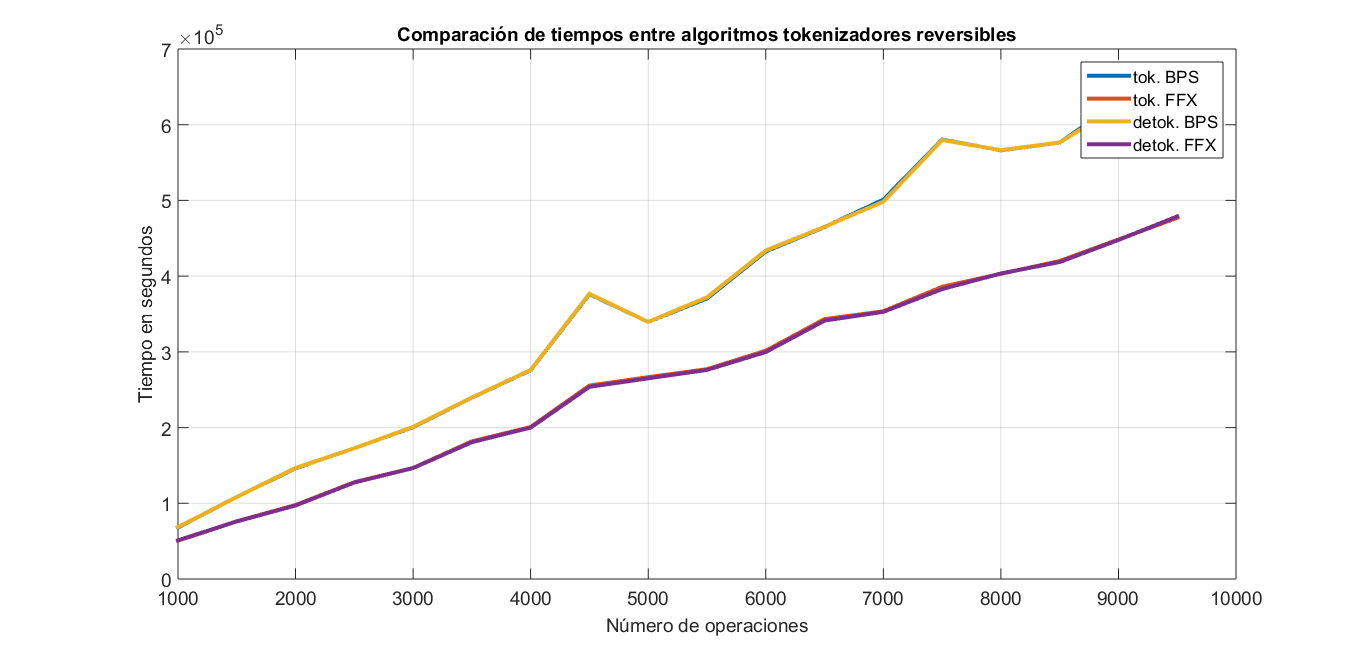
\includegraphics[width=1\linewidth]{estaticos/imagenes/todo_rev.png}
    \caption{Comparación de algoritmos reversibles}
  \end{center}
\end{figure}

Es importante observar que los tiempos de tokenización y detokenización
son tan parecidos, que sus gráficas se sobreponen completamente.

En esta otra se muestra los tiempos de tokenización y detokenización de
TKR, AHR y DRGB mientras el número de operaciones se incrementa.

\begin{figure}[H]
  \begin{center}
    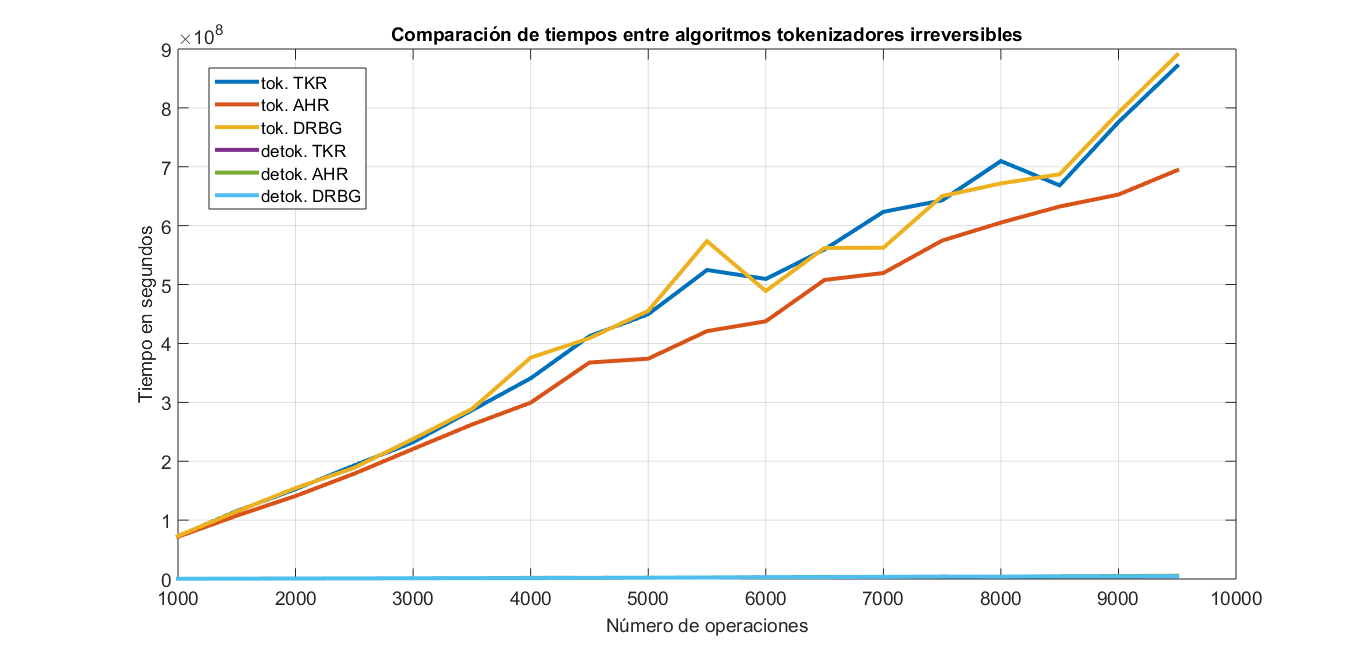
\includegraphics[width=1\linewidth]{estaticos/imagenes/todo_irrev.png}
    \caption{Comparación de algoritmos irreversibles}
  \end{center}
\end{figure}

Aquí es importante resaltar que, si bien el tiempo de tokenización es
considerable (comparándolo con los reversibles), el tiempo de
detokenización es mucho más corto, incluso es menor a los algoritmos
reversibles.
